\documentclass[handout]{beamer} % set [handout] as an option to remove /pause breaks
%\documentclass{beamer}
\usetheme{McMaster}
\beamertemplatenavigationsymbolsempty 
\usepackage{tikz}
\usepackage[export]{adjustbox} % for left/right justifying images
\title{Teaching a Dog to Catalog: An Abbreviated History of Large Language Models and an Inquiry as to Whether They Can Replace Us}
\author{John Fink}
\institute{McMaster University}
\date{October 24, 2023}

% Talk is 2023-10-24 11am, Halifax, Access Conf
% History (briefer than may's talk)
% Definition of terms:
%	"AI"
%	"GAI"
%	LLMs

% Ethical Considerations (maybe put them front and centre, like:
% 	I don't address:
%	Copyright/ethics
%	Pedagogy/academic honesty 
% Difference between *tuning*(including LoRA) and *vector*/document retrieval
% Important LLM (including ChatGPT concepts)
%	context size
%	parameters (7b, 13b, 30b, 65b)
%	Training (Lora, RLHF, few-shot, zero-shot) 
%	Temperature and those other llama.cpp variables (which I think are
%	common to all LLMs)
%	The Prompt
% Other proprietary LLMs (slightly less exasperated sigh)
%	Bard? Anthropic? BERT/RoBERTa?
% Open Source LLMs
% 	Meta's LLaMa
% 	LlaMa Leak
%	Hugging Face
%	Everything else!!!!
%	Non-LLaMa models
% 		StarCoder, RedPajama, etc. etc. etc.
%	Two ways to run local
%		CPU vs GPU
% 		emphasize that CPU is *many factors slower* than GPU
% The Future is Small:
% 	Environmental/other impact of Big Giant Systems
%		Water, electricity, etc
% Altering models:
% 	What is training? 
%	What is fine-tuning?
%	What is ... retreival (RAG? other? find out)
\begin{document}
\begin{frame}
    \maketitle
\end{frame}

\begin{frame}
	John Fink
	
	Digital Scholarship Librarian
	
	McMaster University
\end{frame}




\begin{frame}
	A (series of) disclaimers:
\end{frame}
 
 

 \begin{frame}[plain]
 	\makebox[\linewidth]{
\includegraphics[width=\paperwidth,height=\paperheight]{dontknow}}
 \end{frame}

\begin{frame}{Important things I \textbf{don't} address (much)}
	\begin{itemize}
		\item Copyright
		\pause
		\item Pedagogical implications, including academic integrity
		\pause
		\item Ethics
		\pause
		\item Truth
		\pause
		\item Beauty
		\pause
		\item The state of the world prior to June 12, 2017.
	\end{itemize}
\end{frame}

\begin{frame}
	These are VERY IMPORTANT concepts.
\end{frame}

\begin{frame}
	Why I say "Large Language Model" and not "AI"
\end{frame}

% I tend to be pretty sure that the term "AI" is not useful here, not because it's true or not true, but because it's *unknowable*, at least by current definitions of "Intelligence". 

% Talking dog parable: “TALKING DOG FOR SALE.” The owner took him to the
%backyard and left him with an old Border Collie. The dog looked up and said:
%“Woof. Woof. Hi, I’m Carl, pleased to meet you.”
%The driver was stunned. “Where did you learn how to talk?”
%“Language school,” said Carl, “I was in a top secret language program with the CIA.
%They taught me three languages:
%How can I help you? как я могу вам помочь? 我怎么帮你?”
%“That’s incredible,” said the driver, “What was your job with the CIA?”

%“I was a field operative and the CIA flew me around the world. I sat in a corner and
%eavesdropped on conversations between foreign agents and diplomats, who never suspected I
%could understand what they were saying, and reported back to the CIA what I overheard.
%“You were a spy for the CIA?” said the driver, increasingly astonished.
%“When I retired, I received the Distinguished Intelligence Cross, the highest honor awarded by
%the CIA, and honorary citizenship for extraordinary services rendered to my country.”
%The driver was a little shaken by this encounter and asked the owner how much he %wanted for
%the dog.
%“You can have the dog for $10.”
%“I can’t believe you are asking so little for such an amazing dog.”
%“Did you really believe all that bullshit about the CIA? Carl never left the farm.




\begin{frame}
	So, about 2017...
\end{frame}

\begin{frame}[plain]
	\makebox[\linewidth]{
\includegraphics[width=\paperwidth,height=\paperheight]{attention}}
\end{frame}

% this is the big one. This is what kick-started *everything* we see today. Prior to this, language generators were goofy and easy to spot as being goofy -- think Racter, think Eliza, think Markov chaining. Not going to fool anyone. After this, pow, the gates are busted open. ChatGPT comes out of this, as well as almost every other recent generative AI that you know of. An absolutely fundamental paper that I *cannot understand*.

\begin{frame}{2017-now! Right now!}
	\begin{itemize}
		\item 2017 - "Attention Is All You Need" paper
		\pause
		\item 2018 - "Improving Language Understanding by Generative Pre-Training" paper
		\pause 
		\item 2020 - "Language Models are Few-Shot Learners" paper (GPT-3)
		\pause
		\item 2022 - InstructGPT, and then ChatGPT
		\pause
		\item 2023 - GPT-4
	\end{itemize}
\end{frame}

\begin{frame}[plain]
	\makebox[\linewidth]{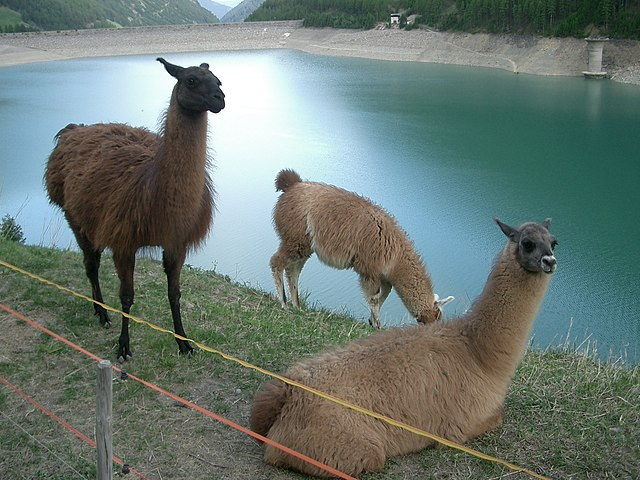
\includegraphics[width=\paperwidth,height=\paperheight]{llamas}}
\end{frame}


\begin{frame}Meta's sort-of open source models
	\begin{itemize}
		\item February 2023 -- Meta's LLaMa v1 released
		\pause
		\item July 2023 -- Meta's LLaMa v2 released
	\end{itemize}
\end{frame}

% February 24th, Facebook introduces LLaMa in a blog post but doesn't freely release how it's made, but it *does* let people have access to it via an application. Of course it was *instantly* leaked, and started an absolute torrent of derivatives. Nearly every locally-runnable model today is based somewhat on the LLaMa original code, which is problematic because it precludes commercial use. There were attempts of to recreate the encumbered LLaMa-v1 in unencumbered models, but in July of 2023 Meta released LLaMa v2, a series of "sort of" open source models upon which a whole  ecosystem is formed.

\begin{frame}
	The immediate, post-2017 frantic present is a weird syncretism of Google and OpenAI, and to a somewhat lesser extent, Meta/Facebook, with other important minor players.
\end{frame} 


\begin{frame}
	A little conversation about the weather.
\end{frame}

\begin{frame}[plain]
	\makebox[\linewidth]{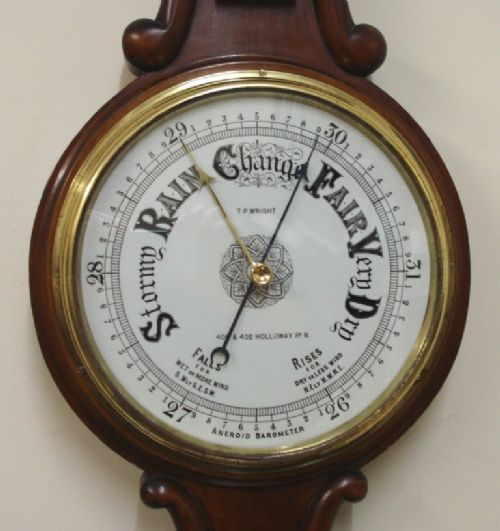
\includegraphics[width=\paperwidth,height=\paperheight]{barometer}}
\end{frame}

\begin{frame}[plain]
	\makebox[\linewidth]{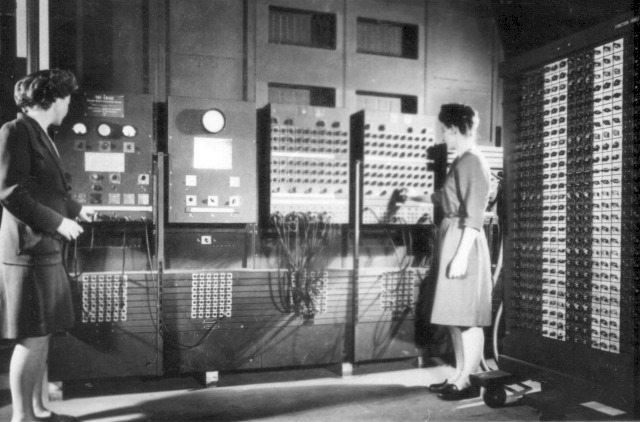
\includegraphics[width=\paperwidth,height=\paperheight]{eniac}}
\end{frame}

% Weather prediction is a lot like language prediction in LLMs. Before the advent of programmable computers, it involved looking at the sky a lot and looking at barometers a lot -- in the 1950s, the early computer ENIAC ran some of the first weather models. Nowadays, we have weather models that are extremely sophisticated and take a lot of computing power to run and can predict the weather many days out. They predict the weather by looking at *current conditions* and extrapolating what *usually happens* from those current predictions, and they're really pretty good at it because there's a lot of data about. This is *eerily similar* to how LLMs/ChatGPT works -- it's not "reasoning" per se, but *predicting* what comes next based on context and what has come previous, and since they have vast, vast amounts of example data -- like the weather models! -- they are pretty good at it. Good enough to fool us, anyway.

\begin{frame}
	Right now, in late 2023, LLMs are sort of midway between weather modeling and...
\end{frame}

\begin{frame}[plain]
	\makebox[\linewidth]{
\includegraphics[width=\paperwidth,height=\paperheight]{eat-up-martha}}
\end{frame}


% Usually LLMs need to run on very beefy graphics cards with lots and lots of VRAM, especially during the training phase. But there are methods to run these models on way more modest hardware and only on the CPU and get decent performance -- of course, not nearly as fast as using GPUs but *very usable* and, more importantly, cheap, cheap, cheap. The raspberry pi in question costs around $100CAD, and *just the graphics card* for a capable GPU-based setup will run about $6000.

\begin{frame}{Important concepts for GPT and other models}
	\begin{itemize}
		\item Context Window and Tokens
		\pause
		\item Few-Shot / No-Shot
		\pause
		\item Parameters
		% GPT-1 117m, GPT-2 1.5b, GPT-3 175b, GPT-4 170t 
		\pause
		\item Training
		\pause 
		\item The Prompt, aka "Programming for English Majors"
		\pause
		\item And the Random Seed.
	\end{itemize}
\end{frame}

\begin{frame}
	\begin{itemize}
		\item Context Window is the "memory" of an LLM
		\pause
		\item And Tokens -- words, roughly -- fill up that "memory"
		\pause
		\item And the \textit{response} also takes tokens.
	\end{itemize}
\end{frame}

% demo https://platform.openai.com/tokenizer

\begin{frame}[plain]
	\makebox[\linewidth]{
\includegraphics[width=\paperwidth,height=\paperheight]{leonard}}
\end{frame}

\begin{frame}{More about tokens and the context window}
	\begin{itemize}
		\item \textit{Tokens} and \textit{context windows} are one of the big limiting factors in nearly every present-day LLM
		% Look up context window size: prior text is 2k for LLaMa, 4k for GPT4 chat, 8k/32k via API. This is short term memory.
		\pause
		\item But \textit{it seems like every day} there is a new paper detailing some new method to get millions of tokens in context
		\pause
		\item So who knows?
	\end{itemize}
	
\end{frame}

\begin{frame}{Few-Shot / No-Shot}
	\begin{itemize}
		\item \textit{Few-Shot} -- a few examples to "teach" an LLM, such as:
		\pause
		\item "I hate it when my phone battery dies." - negative
		\pause
		\item "My day has been great!" - positive
		\pause
		\item "Here is an article." - neutral
		\pause
		\item "This presentation is going fantastic!!!!" - positive(ly optimistic)
		\pause
		\item And \textit{No-Shot} is exactly what you think it is.
	\end{itemize}
\end{frame}

\begin{frame}{Training}
	\begin{itemize}
		\item Usually done on text corpuses
		\pause
		\item The Pile (825GiB), Github, ShareGPT, etc.
		\pause
		\item (cough) books3....
		\pause
		\item And other terms like RLHF (Reinforcement Learning from Human Feedback)
		\pause
		\item The larger the model, the more resources it takes to train or re-train.
	\end{itemize}
\end{frame}

\begin{frame}{Parameters}
	\begin{itemize}
		\item Roughly corresponds to how "Complex" or "Smart" a model is.
		\pause
		\item (...very roughly)
		\pause 
		\item But \textit{definitely} correlates to resources needed to run the model.
		\pause
		\item Which is why, say, GPT-4 (probably 1.7 trillion) requires this....
	\end{itemize}
\end{frame}

\begin{frame}[plain]
	\makebox[\linewidth]{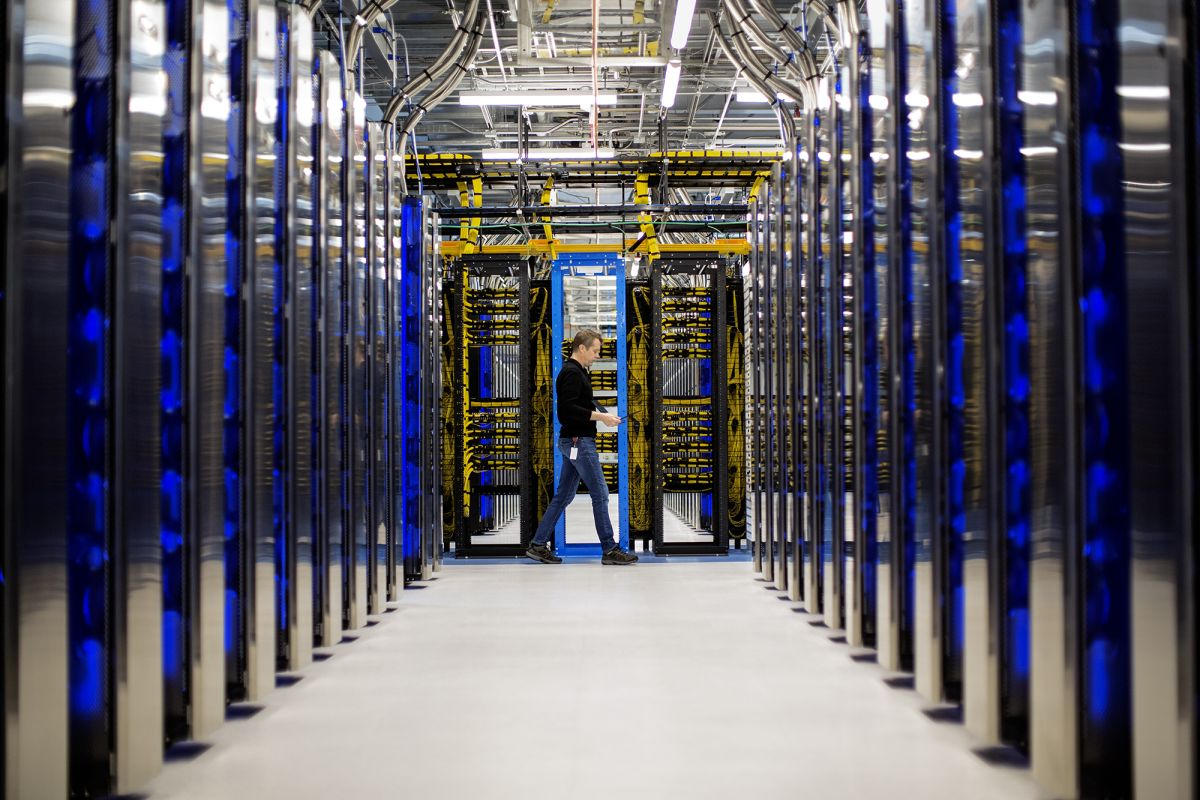
\includegraphics[width=\paperwidth,height=\paperheight]{azure-data-centre}}
\end{frame}

\begin{frame}
	And you can run a 7B model on this....
\end{frame}

\begin{frame}[plain]
	\makebox[\linewidth]{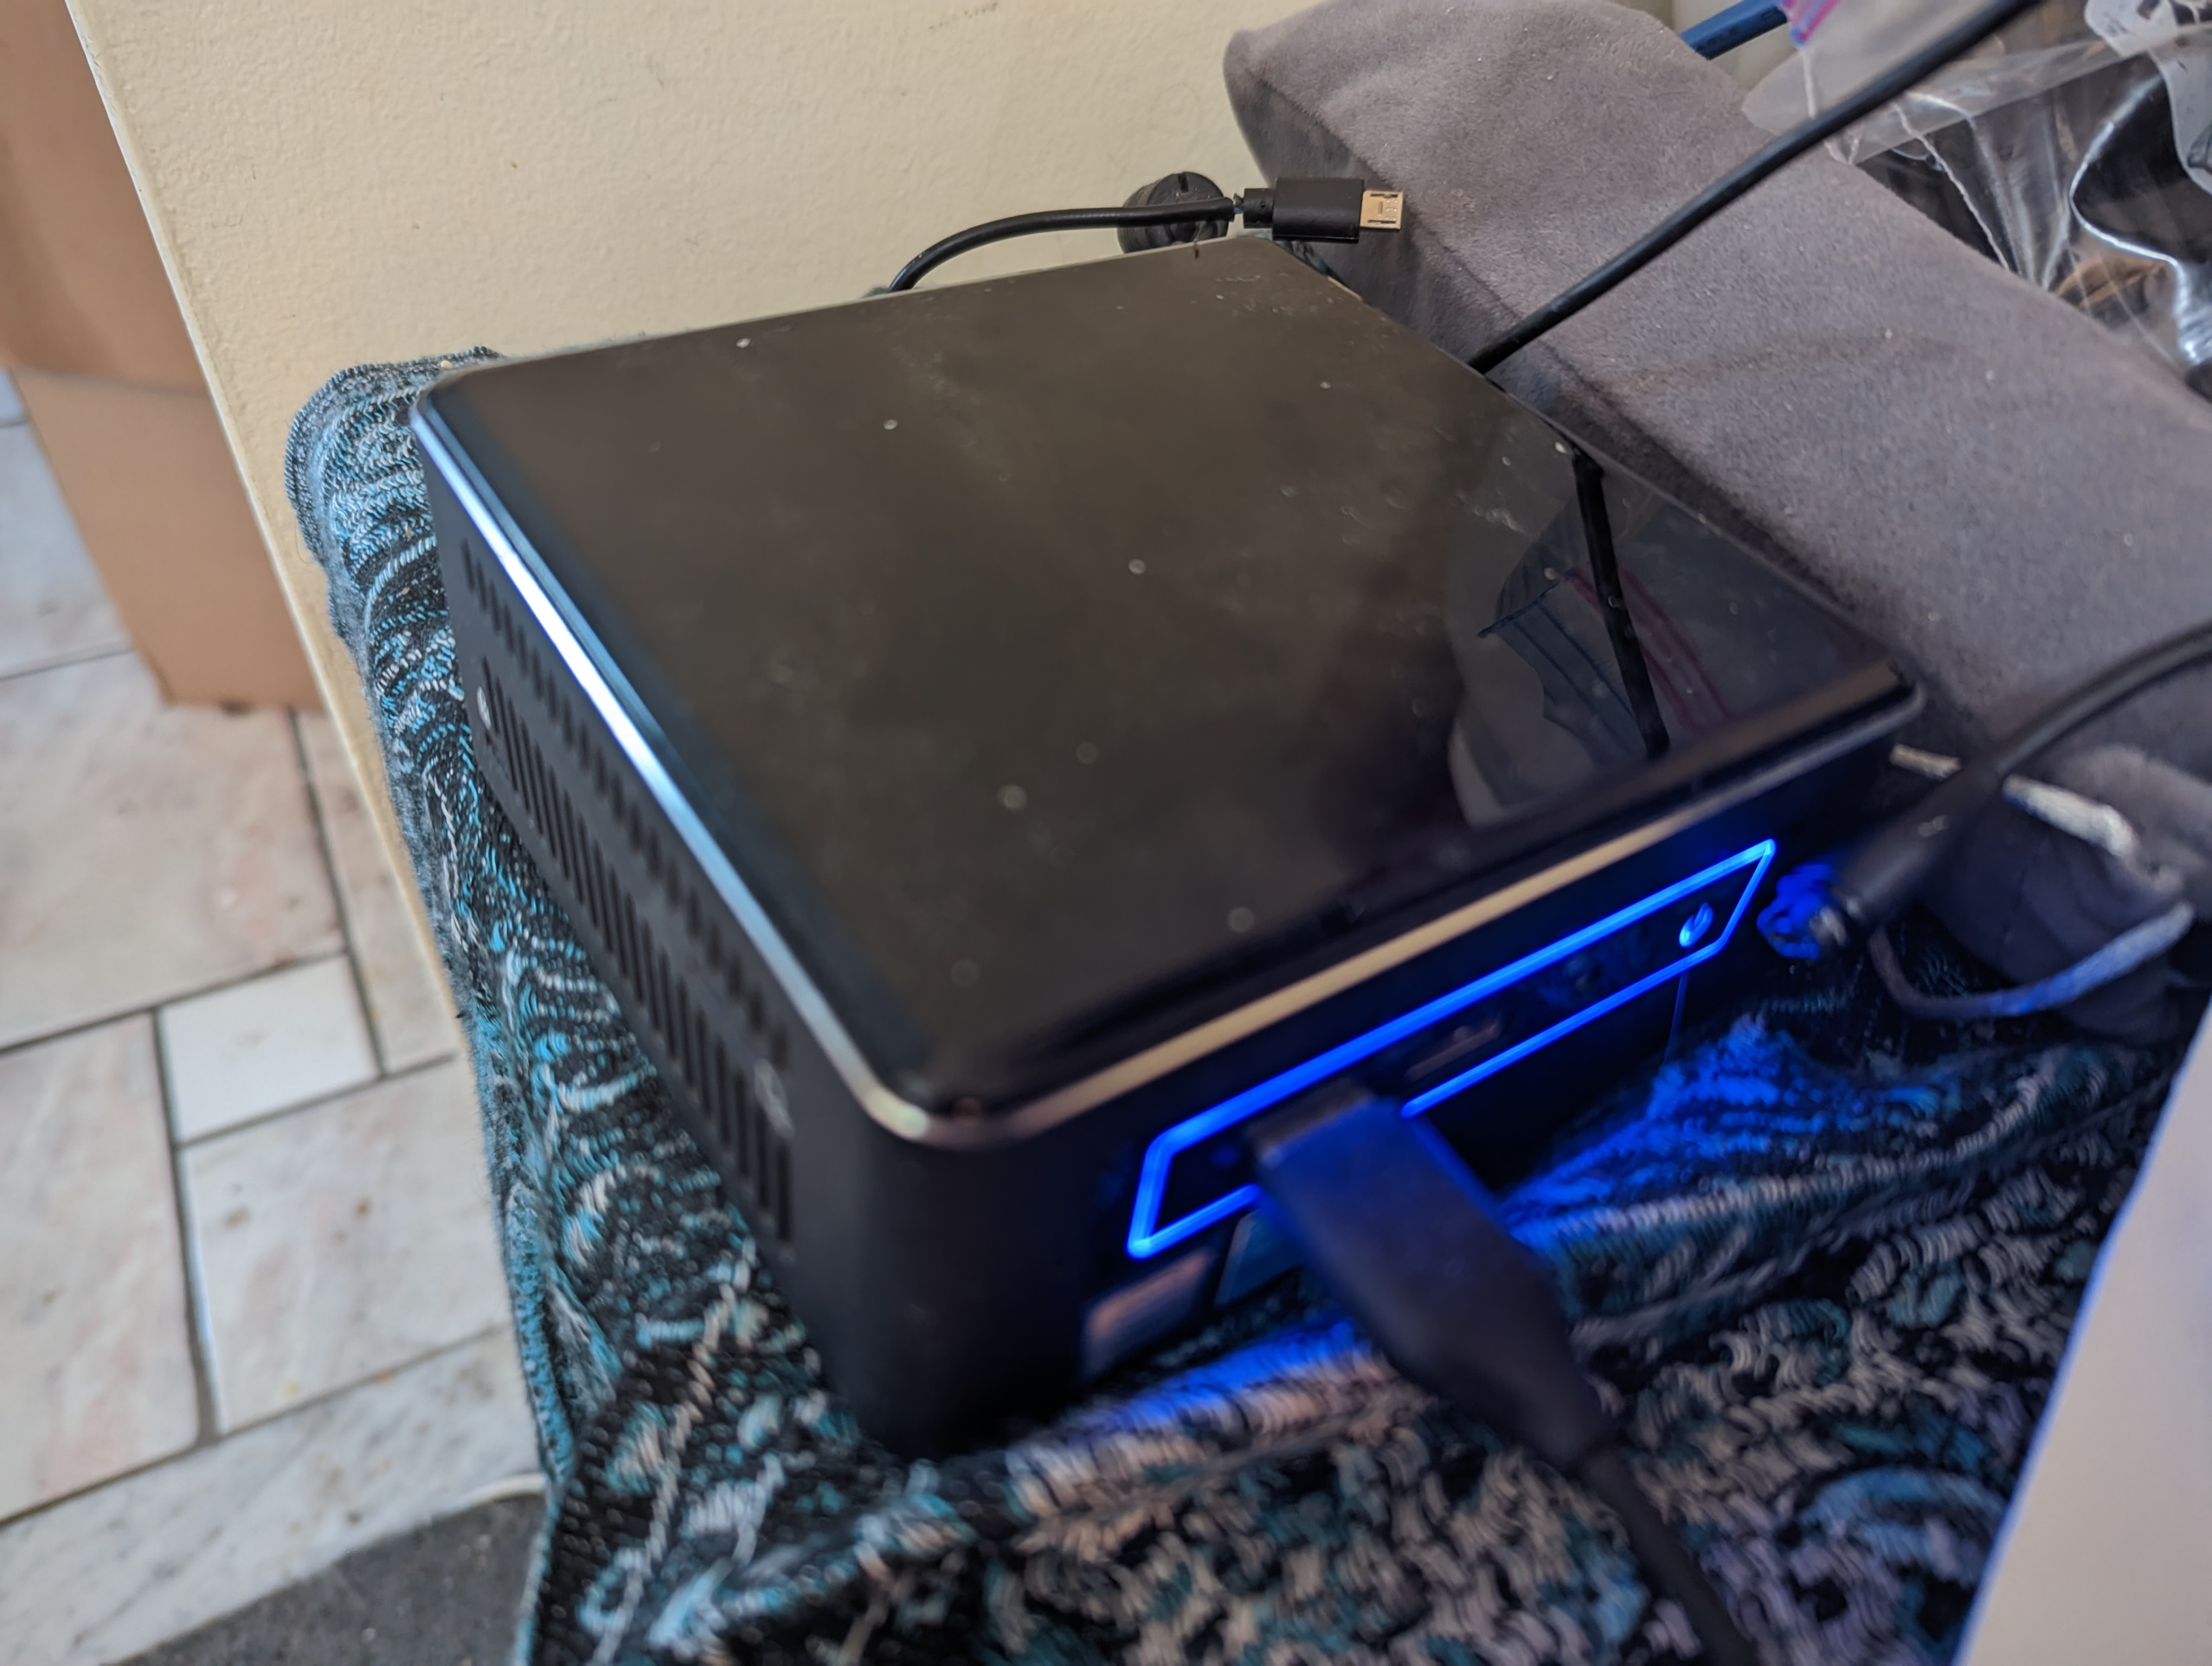
\includegraphics[width=\paperwidth,height=\paperheight]{pfeebe}}
\end{frame}



\begin{frame}
	llama.cpp -- https://github.com/ggerganov/llama.cpp
\end{frame}

\begin{frame}{quantization of models}
	\begin{itemize}
		\item llama.cpp runs on \textit{quantized} models, which is roughly a compression technique that drastically cuts down the size, and more crucially, the processing power needed to run a model.
		\pause
		\item So, Mistral's LLM -- a popular open-source model -- is roughly 15GB unquantized and pretty much requires dedicated GPU to run well, whereas with the most \textit{extreme} quantization, it can get to about 3GB and can run on a reasonably modern smartphone.
		\pause
		\item As running an LLM generally requires fitting the entire model in RAM or VRAM, this can be helpful.
		\pause 
		\item Quantization is like \textit{lossy compression} -- smaller the model, the more tradeoffs, although with less-extreme quantization the differences are fairly negligible.
	\end{itemize}
	
\end{frame}

\begin{frame}{The Prompt}
			Asking the right questions
\end{frame}

\begin{frame}[plain]
	\makebox[\linewidth]{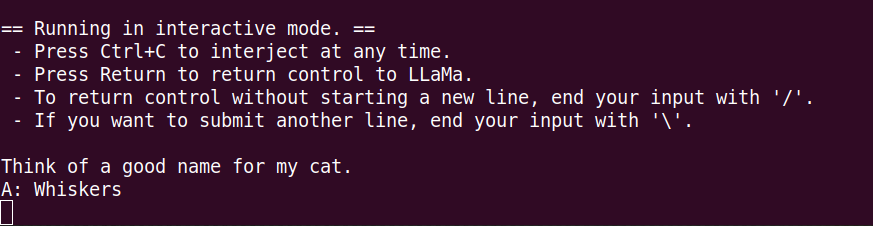
\includegraphics[width=\paperwidth,height=\paperheight]{whiskers}}
\end{frame}

\begin{frame}[plain]
	\makebox[\linewidth]{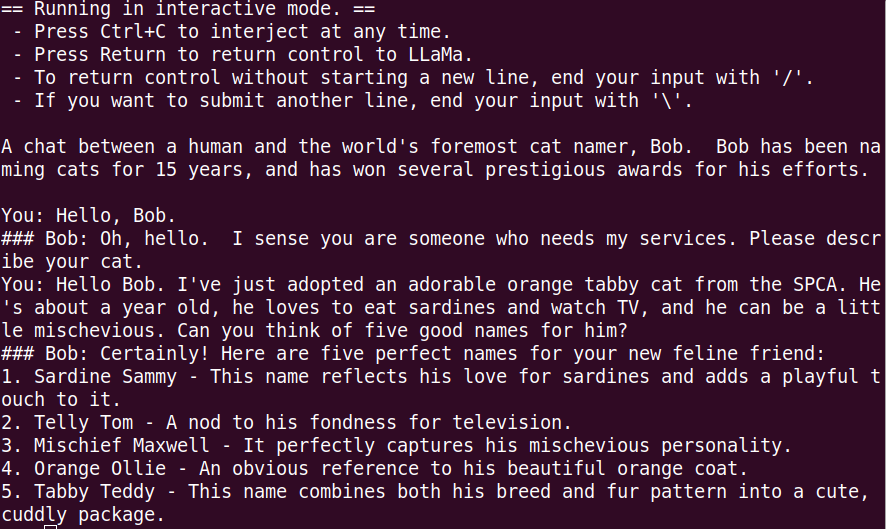
\includegraphics[width=\paperwidth,height=\paperheight]{bob-names-cats}}
\end{frame}


\begin{frame}{teaching an old dog new... dog stuff}
There are roughly \textit{three} ways to get new information into a model.
\begin{itemize}
	\pause
	\item Train from scratch
	\pause
	\item Consulting external sources (Retrieval Augmented Generation et al)
	\pause
	\item Tuning on top of an existing model
\end{itemize}
\end{frame}
	
	
	
\begin{frame}
	Why even do this?
\end{frame}
	
\begin{frame}{Why even do this?}
\begin{itemize}
	\item Running your own models on modest hardware is (or can be):
	\pause
	\item slow
	\pause
	\item (more) inaccurate
	\pause
	\item annoying
\end{itemize}  
\end{frame}

\begin{frame}{Why even do this?}
	The obvious:
	\begin{itemize}
		\item Privacy
		\pause
		\item Environmental Impact
		% A recent study in Joule postulated that within four years AI could rival the countries of Argentina, the Netherlands, or Sweden in total electricity use.
		\pause 
		\item Cost
		
	\end{itemize}
\end{frame}


\begin{frame}
	A \textit{small} model tuned with high-quality information may be more effective than a huge, generic model
\end{frame}


\begin{frame}{Possible applications for libraries}
	OK, so, what about libraries?
\end{frame}

\begin{frame}{Possible applications for libraries}
	\begin{itemize}
		\item Chatbot trained on site-specific reference transactions
		\pause
		\item Pro: A possibly genuinely useful service, especially during off-hours
		\pause
		\item Con: Privacy, hallucinations
	\end{itemize}
\end{frame}

\begin{frame}{Possible applications for libraries}
	\begin{itemize}
		\item Programming-specific model tuned with examples of MARC records.
		\pause
		\item Pro: Public data
		\pause
		\item Con: Complex
		\pause
		\item Con: Maybe only useful for edge cases
		\pause
		\item Con: Will make catalogers mad if it works
	\end{itemize}
\end{frame}

\begin{frame}{Possible applications for libraries}
	\begin{itemize}
		\item Multimodal model (trained on images + text) for image description of unique collections or OCR
		\pause
		\item Pro: Public data, genuinely useful
		\pause
		\item Con: Would still need editing/vetting due to (sometimes hilarious) inaccuracies
		
	\end{itemize}
\end{frame}

\begin{frame}[plain]
	\makebox[\linewidth]{
\includegraphics[width=\paperwidth,height=\paperheight]{ztd}}
\end{frame}

\begin{frame}[plain]
	\makebox[\linewidth]{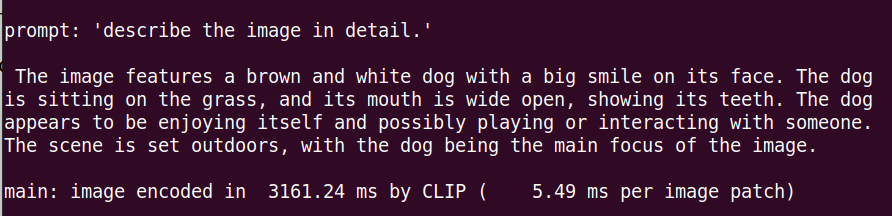
\includegraphics[width=\paperwidth,height=\paperheight]{ztd-description}}
\end{frame}

\begin{frame}[plain]
	\makebox[\linewidth]{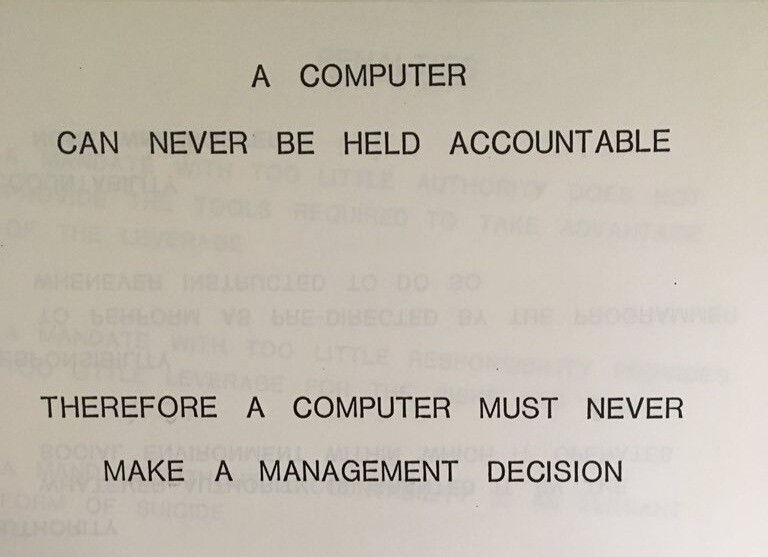
\includegraphics[width=\paperwidth,height=\paperheight]{a-computer}}
\end{frame}

\begin{frame}[plain]
	\makebox[\linewidth]{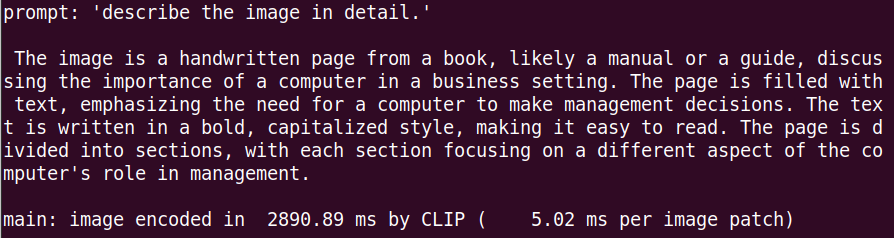
\includegraphics[width=\paperwidth,height=\paperheight]{a-computer-description}}
\end{frame}

\begin{frame}
	%this is always the last slide
	Any questions?\\ 
	jfink@mcmaster.ca\\
	
\includegraphics[left, height=4mm]{mastodon} \hspace{1mm}  https://glammr.us/@jbfink
	
\end{frame}

\end{document}
